%%%%%%%%%%%%%%%%%%%%%%%%%%%%%%%%%%%%%%%%%%%%%%%%%%%%%%%%%%%%%%%%%%%%%%%%%%%%%%%
% Active Learning Machine Learning Methodology %%%%%%%%%%%%%%%%%%%%%%%%%%%%%%%%
% %%%%%%%%%%%%%%%%%%%%%%%%%%%%%%%%%%%%%%%%%%%%%%%%%%%%%%%%%%%%%%%%%%%%%%%%%%%%%
%
% Points to mention:
%   * Active learning frameworks are a means by which to generate the most valuable training data set, on the fly.
%   * The search space of materials is not a continous space but a discrite array of individual structures
%
% TODO:
%%%%%%%%%%%%%%%%%%%%%%%%%%%%%%%%%%%%%%%%%%%%%%%%%%%%%%%%%%%%%%%%%%%%%%%%%%%%%%%



% ################################# Paragraph #################################
% %%%%%%%%%%%%%%%%%%%%%%%%%%%%%%%%%%%%%%%%%%%%%%%%%%%%%%%%%%%%%%%%%%%%%%%%%%%%%
% General intro to AL scheme
% Basic gist, i.e. define our candidate space of materials to explore within (we do this by looking taking all structurally unique systems in DBs)
% To start the AL we take the few systems that have DFT calcs (more generally we can just choose random structures)
% We then build a surrogate model (GP, initially really bad) to predict the stability of the entire candidate space
% %%%%%%%%%%%%%%%%%%%%%%%%%%%%%%%%%%%%%%%%%%%%%%%%%%%%%%%%%%%%%%%%%%%%%%%%%%%%%
% | - Paragraph start
%
Here, we present an active learning accelerated methodology for discovering novel and stable crystal polymorphs.
%
Our approach is based on the principles of surrogate-models paired with an active learning framework,
whereby a simple surrogate model is trained on a set of candidate materials by iteratively sampling structures that are predicted to be low in energy.
%
% COMBAK Does the hansen2019atomistic paper really demonstrate structural optimizations? Double check
Active learning frameworks utilizing surrogate models have been demonstrated to successfully speed up materials discovery for alloy nanoparticles \cite{Jennings2019}, structural optimizations \cite{hansen2019atomistic}, and transition-state searches \cite{torres2019low}, as well as adaptive approaches for global optimization \cite{VanDenBossche2018}.
%
% TODO All global optimization papers go here
More generally a large body of work has been devoted to the problem of polymorph discovery and global optimization.
%
These methods are inherintly limited by the curse of dimensionality associated with the highly dimensional potential energy surface (PES).
%
An alternative method to exploring the PES through global optimization routines is to prepare a static list of candidate structures that will be searched through.
%
This method relies on being able to prepare candidate structures that are likely to be low energy.
%
Since nature tends to form symmetric structures, we use this intuition to build a candidate set of structures that have symmetry built in.
%
The methodology consists of two steps (outlined in figure \ref{fig:all_diagram}).
%
The first step is the generation of the candidate space,
which defines the inclusive list of all crystal structures to be screened through during the search routine.
%
Since the initial candidates determines which structures that can ultimately be discovered, it is crucial to define a candidate space that is sufficiently diverse.
%
% TEMP Say more
The second part of the algorithm is the iterative active learning algorithm.

% | - __old__
% Our machine learning accelerated materials discovery method proceeds through the following steps:
% First, the dataset of candidate materials is constructed.
% This data set will define the totality of materials that will be considered by the search algorithm,
% this is done because the search space of materials is not a continous space but a discrite array of individual structures.
% Next, the dataset of materials is transformed into a vectorial representation by using a fingerprinting method that encodes the relevent chemical and structural information.
% __|

% __|


% ################################# Paragraph #################################
% %%%%%%%%%%%%%%%%%%%%%%%%%%%%%%%%%%%%%%%%%%%%%%%%%%%%%%%%%%%%%%%%%%%%%%%%%%%%%
%
% %%%%%%%%%%%%%%%%%%%%%%%%%%%%%%%%%%%%%%%%%%%%%%%%%%%%%%%%%%%%%%%%%%%%%%%%%%%%%
% | - Paragraph start
% TODO PENDING Ask @Ankit for these numbers
% The MP project number should be correct, but the OQMD number might be wrong
% MP{AB2: 3995, AB3: 2849} | OQMD{AB2: 533, AB3:20915}
In Schema \ref{fig:all_diagram} we show the overall process with the integrated active learning loop.
% NUMBER
The structures that comprise the candidate data sets for \IrOtwo and \IrOthree were constructed by parsing for all bulk \ABtwo and \ABthree structures in both the Materials Project\cite{Jain2013} and OQMD\cite{Kirklin2015} databases
(in total 4528 \ABtwo and 23764 \ABthree entries).
%
Structurally redundant systems were then removed via a space-group based structural classification scheme developed by Jain \latin{et al.} \cite{Jain2018},
whereby structural uniqueness is defined by the element-nonspecific stoicheometry (\ABtwo, \ABthree, etc.), spacegroup symmetry and wyckoff positions of the atoms within the unit cell.
%
% COMBAK
This filtering step consideribly reduces the pool of candidates to 697 and 259 structures for the \ABtwo and \ABthree stoicheometries;  % NUMBER
this is a prime indication of the lack of structural diversity in the OQMD and MP databases.
% NUMBER
Furthermore, only bulk structures containing $\leq$ 75 atoms were included in the final candidate pool to reduce the computational expense of the DFT compuations
(further reducing the candidates spaces to 567 and 256 \ABtwo and \ABthree structures respectively).
%
Next, iridum and oxygen were subsituted for the A and B sites, respectively,
this was then followed by a crude isotropic expansion/contraction of the unit cell to accommodate the atomic radii of iridium and oxygen.
% NUMBER
Because of the relitively small size of the candidate space and because we wish to validate our methods fully, we performed bulk relaxations for all 823 structures in the candidate space.
%
Of the 823 structures, 736 were able to be fully optimized, while 87, primarily \ABtwo structures were not able to be converged for a variety of convergence issues stemming from highly volumnous and unphysical initial structures.
%
The resulting candidate space was composed of 487 \IrOtwo and 249 \IrOthree structures, all of which have unique space group/Wyckoff combintations, ensuring their structural uniquness.
%
See section (SI Bulk polymorph DFT optimization) for further details on the computational methodology used to relax the bulk structures.
%
While size of this dataset is not particularly large, it will serve the purpose of demonstrating the polymorph discovery routine as a proof of concept.
%
Additionally, the dataset is small enough that computing all of the structural candidats with \latin{ab-initio} DFT is tractable, thus allowing us to validate the performance of the model.
% __|


% ################################# Paragraph #################################
% %%%%%%%%%%%%%%%%%%%%%%%%%%%%%%%%%%%%%%%%%%%%%%%%%%%%%%%%%%%%%%%%%%%%%%%%%%%%%
%
% %%%%%%%%%%%%%%%%%%%%%%%%%%%%%%%%%%%%%%%%%%%%%%%%%%%%%%%%%%%%%%%%%%%%%%%%%%%%%
% | - Paragraph start
The candidate data set was featurized using the Voronoi tessellation fingerprinting scheme developed by Ward \latin{et al.} \cite{Ward2017} which produces a 271 length feature vector for each material that is invariant to isotropic expansions/contractions of the lattice and to a degree, insensitive to the exact atomic coordinates of the atoms.
%
% How many columns of the 271 are redundant if stoich and composition are frozen
Herein, we apply our active learning model to the \IrOtwo and \IrOthree spaces separately, because we are interested in the most stable polymorphs at each stoichiometry.
%
Contraining the stoicheometry per application of the AL algorithm further reduces the 271 length  feature vector to 101 non-zero variance features,
significantly reducing the dimensionality of the features.
%
% COMBAK TODO How much of the variance is captured by the PCA analysis
Further dimensionality reduction is achieved via a principle component analysis (PCA) \cite{Tipping1999}, which was used to reduce the remaining 101 features to 11.
%
The active learning algorithm proceeds through iterative generations of ML training, prediction, and acquisition steps that are visualized in figure \ref{fig:iro2_al}.
%
% COMBAK Did I get all of the important features of GP here? @Jose
To start, we utilized Gaussian process (GP) regression with gaussian (or RBF) kernels as implemented in the CatLearn\cite{hansen2019atomistic,CatLearn_Repo} package for atomistic machine learning applications, and used it to train a regression model on a small seed set of DFT formation energies from randomly selected structures in the candidate space.
%
% NOTE I've introduced the aquis. crit. with the GP uncertainty before talking about aquis. in more detail, need to restructure
Herein, we utilized Gaussian process regression because they are highly flexible regression models which have built-in error quantification for each prediction.
%
The model is then used to predict the formation energies of the entire candidate space.
%
This predicted energy landscape is then used to select the next systems to calculate via a aquisition function, which defines a fitness score for each system, and systems that minimize this quantity are then selected.
%
Herein, we use the so-called GP-UCB acquisition function
%
% TODO Should we change the sigma to an uncertainty term? (more precise/direct)
% The name for this kind of acquisition is calld GP-UCB (Upper confidence bound)
% https://www.cse.wustl.edu/~garnett/cse515t/spring_2015/files/lecture_notes/12.pdf
\begin{equation}
    U = \mu - \kappa \sigma,
\end{equation}
%
where $\mu$ and $\sigma$ is the predicted mean and uncertainty of the formation energy,
and $\kappa$ is a free parameter to tune the relative weighting between exploiting low formation energy systems (small $\kappa$) and exploring high uncertainty regions of the candidate space (large $\kappa$).
%
Here, $\kappa$ is set to $1$ which equally weights the energy and uncertainty.
%
In this work we attempt to trade off exploitation and exploration by weighting the predicted formation energy and the associated uncertainty to bias systems that are both low energy and high uncertainty.
%
% TODO N is used into mean number of atoms (FIX)
Once ranked, the N systems that minimize the acquisition function are selected for full DFT calculations, which are included in the training data of subsequent AL generations.
%
Here we chose a bin size (N) of 5, the value of the bin size ($N$) determines how many structures are selected for DFT calculations,
and as such, determines the degree of parallization of the routine.
%
The optimal value of $N$ depends on the computational resources available, as small values of N result in an algorithm that is slow, as every DFT calculation is performed serially.
%
% TODO: Is this statement true?
Larger values of N speed up the active-learning algorithm, but leads to a higher number of DFT calculations performed before convergence.
%
Although initially unique, the structures in the candiate often relax into one another over the course of the DFT optimization, introducing duplicate structures in the post-DFT structures.
%
These duplicate structures are removed during each generation of the AL algorithm, leaving only a single instance of lowest energy in the candidate pool.
%
The coordination characterization function (CCF) based methodology to quantify the simalarity between structures was used to identify and remove duplicate structures.\cite{Su2017}
%
% COMBAK We are discussing alternative convergence criteria, or whether to even have convergence criteria here
The AL loop proceeds until convergence is achieved, which here is chosen to be the generation at which the structures within the range of metastability, here taken as 0.1 eV/atom, are unchanging over three consecutive generations.
% __|



% | - Figure | Active Learning Algorithm **************************************
\begin{figure*}[!htb]
\centering
\makebox[\textwidth][c]{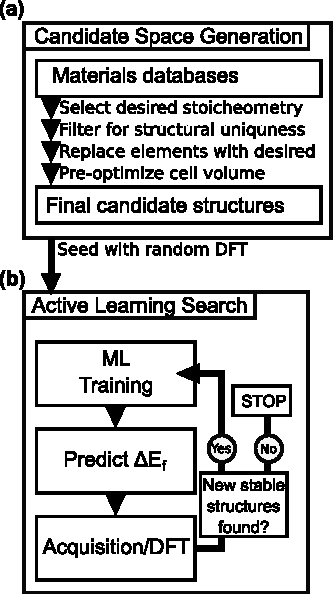
\includegraphics
  {02_figures/al_diagram/Surrogate_model_mine.pdf}
  }
\caption{\label{fig:all_diagram}
% Probably better to keep this caption really concise and refer to the text
Process flow diagram for the active learning accelerated algorithm. The procedure is composed of (a) generation of the candidate set of considered crystal structures constructed from DFT materials databases and (b) iterative active learning surrogate search of the candidate space.
}
\end{figure*}
% __|
